\chapter{Open surface code simulations}\label{ap:oopsurfacecode}

Object-oriented programming is a class of programming based on the concept of \emph{objects}. Each object can contain data in the form of object \emph{attributes}, and code in the form of object \emph{methods}. A significant feature of these objects is that they can interact with themselves or other objects, modifying their own or other object's attributes with their methods. More often than not, these objects are \emph{class}-based, which means every object are \emph{instances} of classes. With the purpose of analyzing the various types of decoders in the thesis, we have created an object-oriented programming package for simulating, decoding, and visualizing a surface code, written in Python3, dubbed \emph{OpenSurfaceSim}. The package consists of the base classes \codefunc{qubit} and \codefunc{stabilizer}, which are the base physical elements of a surface code, and several main classes that construct, simulate and decode the surface code. 

Within the graph representation $G(V,E,F)$ (Section \ref{sec:toricgraph}), elements $v\in V$ and $f\in F$ are now instances of \emph{sub-classes} of the \codefunc{stabilizer} class. A subclass is a class that inherits all methods and attributes of the parent class, while also new attributes and methods can be defined. Recall that vertices are equivalent to ancillary qubits with star operators measurements, and faces are equivalent to ancillary qubits with plaquette operators measurements. For boundary vertex elements $V_\delta$ and non-stabilizer vertex elements $V_\omega$, a different subclass can be defined in the same way. Attributes $var$ of a vertex $v$, an instance of a (sub)class of the \codefunc{stabilizer} class are denoted with $v.var$. For the primal and dual graphs $G_V(V,E_V), G_F(F,E_F)$, an instance of the \codefunc{qubit} class is equivalent to an edge in both $E_V$ and $E_F$. Attributes $var$ of an edge $e$, an instance of a (sub)class of the \codefunc{qubit} class are denoted with $e.var$. 

Using these base classes, we can construct a surface code and perform operations to simulate errors and decoders. The main class types necessary for such a simulation are:
\begin{itemize}
    \item \codefunc{Graph}: Classes containing the geometrical information necessary to construct a surface code in the graph representation, by creating instances of the \codefunc{qubit} and \codefunc{stabilizer} classes and linking them appropriately.
    \item \codefunc{Error}: Classes containing the methods and attributes affiliated with the error models that are applied to the elements of the graph during a simulation.
    \item \codefunc{Decoder}: Classes containing the methods or algorithms that can decode a given graph with some error. 
\end{itemize}
Each main class type can define new attributes or methods at the \codefunc{qubit} and \codefunc{stabilizer} classes, such that variables specific to a graph type, error model, or decoder are available at the base object level. This allows for any attribute required for a particular type of lattice, error model, or decoder to be directly stored at the qubit's or stabilizer's object level. 

For new users, \emph{OpenSurfaceSim} provides an interactive GUI for guided step-by-step visualization of the simulated surface code itself and the used decoder. The user can quickly get a detailed understanding of the underlying mechanics of the code and the decoder. For advanced users, the package can serve as a tool to analyze and benchmark decoders. The package contains tools for code threshold simulations, which is the numeric used to compare different decoders. Scripts  for batched processes on a computation cluster are included as well. Furthermore, heuristics and results from different simulations can be compared easily. Finally, the class-based structure of the package decreases the complexity of creating new types of \codefunc{Graph}, \codefunc{Error}, or \codefunc{Decoder} classes, which should allow for contributions in an open-sourced environment. 

The repository of \emph{OpenSurfaceSim} can be found at \href{https://github.com/OpenSurfaceSim}{GitHub}. 

\begin{figure}[htbp]
    \centering
    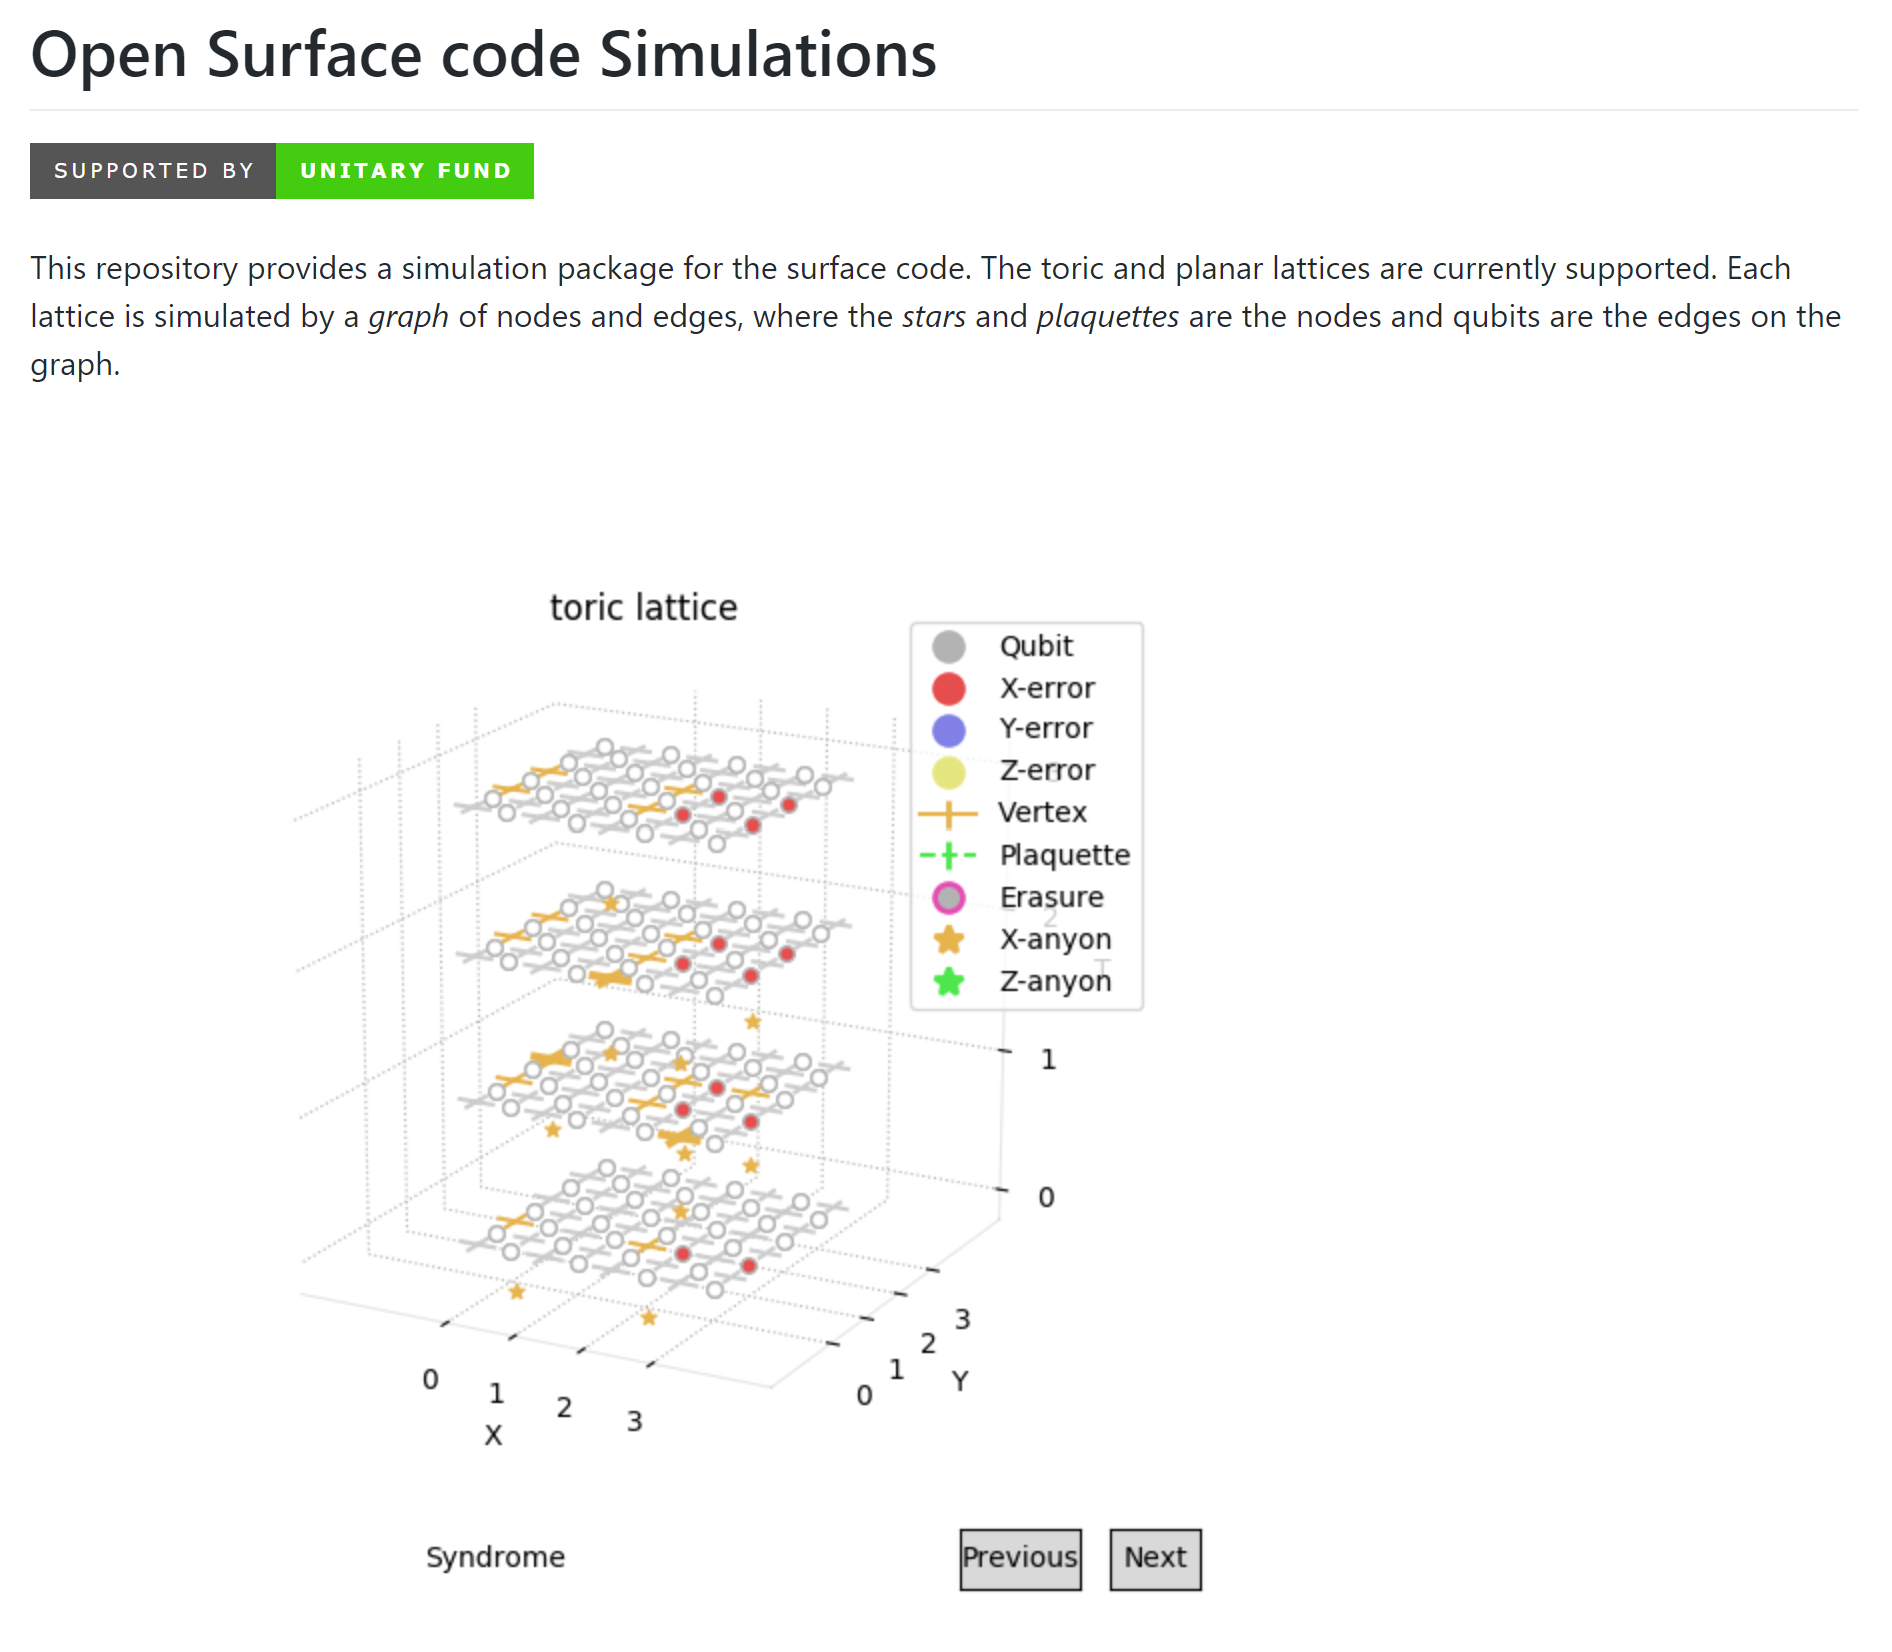
\includegraphics[width=0.9\textwidth]{fig/opensurfacesim.png}
    \caption{The GitHub repository for \emph{OpenSurfaceSim}.}
    \label{fig:opensurfacesim}
\end{figure}
% For example, we can create instructions for creating a toric code or a planar code as sub-classes of the \codefunc{Graph} class. This allows for the data pass-through for different types of graphs, error models and decoders to be identical. For example, if we decide \emph{erasure} noise to be the applied noise model, the locations of erased qubits is an extra variable. In a non object-oriented environment, this would be done by defining a list of locations which needs to be fed, along with other information, to the \codefunc{decoder} object. For independent Pauli noise, maintaining this extra list is not necessary. This would mean that for every combination of graph, error, and decoder types a different data pipeline is necessary. Storing a boolean for the state of erasure as an attribute \codefunc{qubit.erased} allows for streamlining this data pass-through, as we only pass the \codefunc{qubit} and \codefunc{stabilizer} instances to the decoder class. It is thus not required to declare any new data objects. Dividing elements of the simulator in these main classes thus allows for interchangeability between main class types. This also decreases the complexity of creating a new main class type to simulate in a new environment. 






% \section{Showcase}